\section{Implementacija opšteg AST}
\label{sec:ImplementationMyAST}

Implementacija prati hijerarhije opisane u poglavlju \ref{chp:MyAST} kroz mehanizam nasleđivanja. Svaki tip čvora je implementiran kao zasebna klasa koja direktno ili tranzitivno nasleđuje apstraktnu klasu \texttt{ASTNode}. Klase koje čine apstrakciju zajedno sa njihovom hijerarhijom se može videti na slikama \ref{fig:UMLASTNode1}, \ref{fig:UMLASTNode2} i \ref{fig:UMLASTNode3}. 

\begin{figure}[h!]
\centering
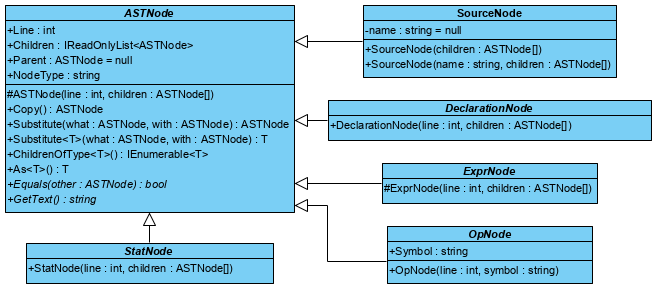
\includegraphics[scale=0.7]{images/uml/ASTNode.png}
\line(1,0){450}\\
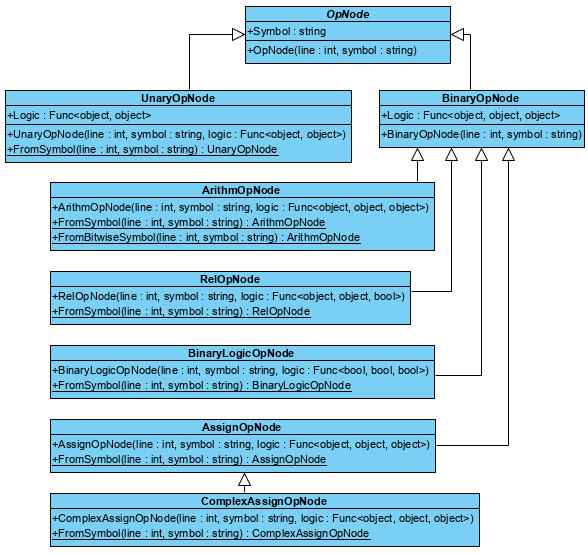
\includegraphics[scale=0.7]{images/uml/OperatorNode.png}
\caption{UML klasni dijagram opšte apstrakcije (deo 1).}
\label{fig:UMLASTNode1}
\end{figure}

\begin{figure}[h!]
\centering
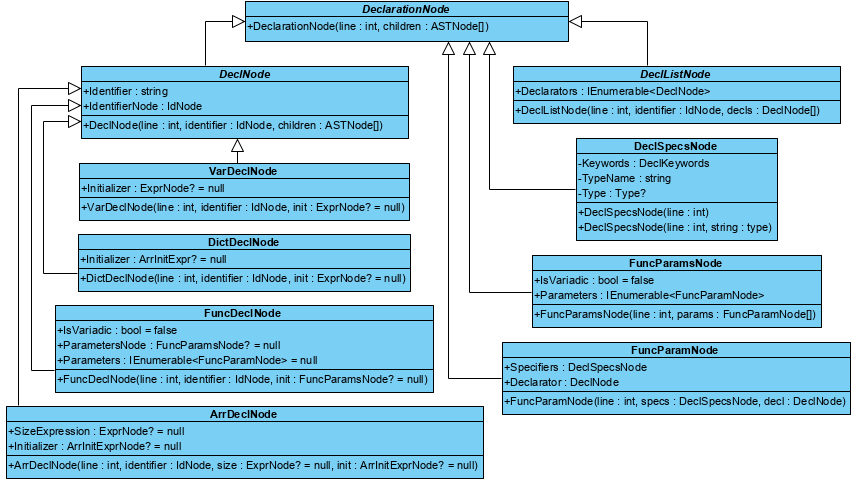
\includegraphics[scale=0.7]{images/uml/DeclarationNode.png}
\caption{UML klasni dijagram opšte apstrakcije (deo 2).}
\label{fig:UMLASTNode2}
\end{figure}

\begin{figure}[h!]
\centering
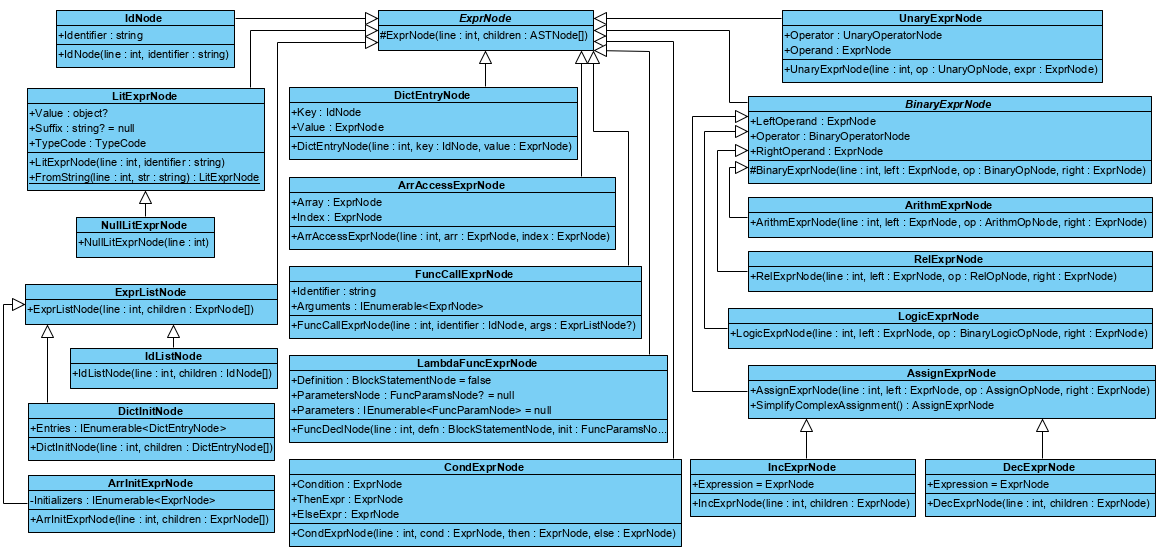
\includegraphics[scale=0.55]{images/uml/ExpressionNode.png}
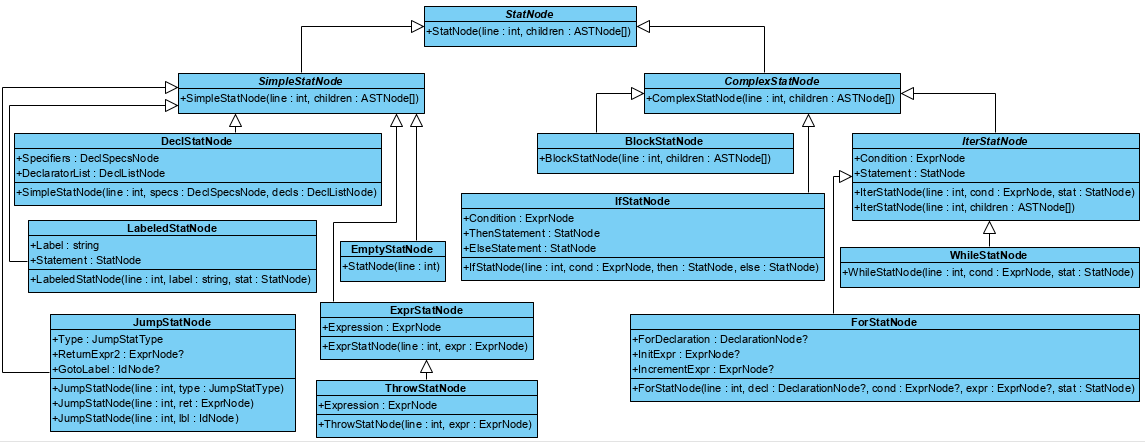
\includegraphics[scale=0.55]{images/uml/StatementNode.png}
\caption{UML klasni dijagram opšte apstrakcije (deo 3).}
\label{fig:UMLASTNode3}
\end{figure}

Jednom kreirani AST čvor je \emph{nepromenljiv}, što znači da je i ceo AST nepromenljiv --- ne mogu se dodavati ili uklanjati deca čvorovima u stablu. Međutim, moguće je klonirati AST čvorove ili vršiti zamenu određenog podstabla drugim podstablom ne menjajući original tako što se vraća izmenjena kopija originala. Svaki AST čvor se može porediti po jednakosti sa drugim AST čvorom po intuitivnoj logici poređenja pruženom kroz predefinisane operatore poređenja. Dostupne su i ekstenzije koje omogućavaju serijalizaciju stabla u JSON format.

Pored implementacije klasa koje predstavljaju AST čvorove, kreiran je i javno dostupni način za obilazak AST putem obrazca posetilac kroz apstraktnu klasu \texttt{BaseASTVisitor<TResult>}. Ova klasa ima implementirane javne virtualno predefinisani metod \texttt{TResult Visit(ASTNode node)} jednog argumenta za svaki mogući tip koji nasleđuje tip \texttt{ASTNode}. Svi ti metodi su definisani tako da se pozove metod \texttt{VisitChildren(ASTNode)} koji će posetiti svu decu trenutnog čvora. Svaki naredni rezultat poziva metoda \texttt{Visit()} za svako dete se agregira pozivanjem metoda \texttt{TResult AggregateResult(TResult curr, TResult next)} koji podrazumevano samo vraća \texttt{next}. Dodatno, moguće je predefinisati metod \texttt{bool ShouldVisitNextChild(ASTNode node, TResult curr)} koji određuje da li je potrebno prekinuti posećivanje pre nego što se posete sva deca. Ovaj metod se poziva svaki put pre nego što se poseti dete i podrazumevano vraća \texttt{true}. \texttt{BaseASTVisitor} klasa je u implementaciji korišćena za kreiranja graditelja simboličkog izraza od sintaksičkog stabla izraza kao i evaluatora takvog stabla izraza. 

Adapteri ili graditelji se koriste kao spona između stabla parsiranja za konkretni programski jezik i opšte AST apstrakcije. Uloga adaptera je da od stabla parsiranja kreiraju opšti AST. Kako bi se pružio ujednačen način za kreiranje adaptera, pružena su dva interfejsa prikazana na slici \ref{fig:ImplBuilderInterface}.

\begin{figure}[h!]
\centering
\begin{lstlisting}
public interface IAbstractASTBuilder
{
    ASTNode BuildFromSource(string code);
}

public interface IASTBuilder<TParser> : IAbstractASTBuilder where TParser : Parser
{
    TParser CreateParser(string code);
    ASTNode BuildFromSource(string code, Func<TParser, ParserRuleContext> entryProvider);
}
\end{lstlisting}
\caption{Interfejs graditelja opšteg AST od stabla parsiranja.}
\label{fig:ImplBuilderInterface}
\end{figure}

Postupak kreiranja AST za dati izvorni fajl se sastoji iz više koraka. Prvo se izvlači ekstenzija izvornog fajla. Zatim se putem refleksije pronalazi klasa koja implementira interfejs \texttt{IAbstractASTBuilder} i ima u sebi prisutan atribut \texttt{ASTBuilderAttribute(string)}\footnote{Atributi u C\#-u su deklarativni tagovi (nalik na anotacije u Java programskom jeziku) koji se koriste da se raznim elementima pridruže informacije dostupne u toku prevođenja. Ti elementi mogu biti klase, metode, osobine itd. Atributi se definišu kao klase i mogu imati polja i konstruktore s tim što vrednosti atributa moraju biti poznate za vreme prevođenja --- konstante.}
čija se niska poklapa sa ekstenzijom izvornog fajla. Naposletku se kreira instanca pronađene klase i, na osnovu toga što implementira interfejs \texttt{IAbstractASTBuilder}, poziva se metod \texttt{BuildFromSource()} za sadržaj izvornog fajla.

Dedukovani adapter implementira uvek \texttt{IASTBuilder} interfejs na osnovu tipa parsera koji je generisao ANTLR alat za gramatiku konkretnog programskog jezika. Metod \texttt{CreateParser()} instancira parser odgovarajućeg tipa. Razlog zašto ovaj proces nije uniforman je taj što se pre kreiranja parsera uvek kreira i lekser koji prvi dobija tok podataka pa se tek onda kreira parser. Dodatno, prilikom kreiranja parsera se definiše i pravilo gramatike od kojeg parser kreće (tzv. \emph{ulazno pravilo}, engl. \emph{entry rule}) koje je specifično za programski jezik. Stoga je nemoguće kreirati jedinstveni niz operacija koji će kreirati svaki parser pa se to radi prilikom implementacije adaptera. 

Predefinisani metod \texttt{BuildFromSource()} interfejsa \texttt{IASTBuilder} treba da obiđe stablo parsiranja počev od pravila koje se dobija pozivom funkcije prosleđene kao drugi argument za dati tip parsera. Ovo je generalizacija kreiranja parsera i na prvi pogled izgleda suvišno jer, pošto se parsira validan izvorni k\^od, mora se uvek krenuti od podrazumevanog ulaznog pravila za konkretni programski jezik. Međutim, ovaj način kreiranja AST je pogodan prilikom testiranja jedinica koda, jer ukoliko se npr. testira generisanje AST od izraza, nije potrebno pisati čitave funkcije sa naredbama samo da bi se testiralo generisanje apstrakcije izraza, već je moguće samo navesti izraz i instrukovati adapter da kreira parser tako da on počne od pravila koje definiše izraz.
